\section{Анализ алгоритма}

\subsection{Принцип работы}

Алгоритм является поиском элемента в массиве.
Программа:
\begin{enumerate}
    \item Выделяет память под массив, инициализирует генератор случайных значений;
    \item Заполняет массив случайными числами;
    \item Ищет элемент с определенными настройками \textit{OpenMP}.
\end{enumerate}

Результатом поиска является индекс элемента в массиве.
Поиск осуществляется последовательно.

Временная сложность алгоритма $O(n)$, где $n$ -- число элементов в массиве.


Блок-схема алгоритма выглядит следующим образом:\\
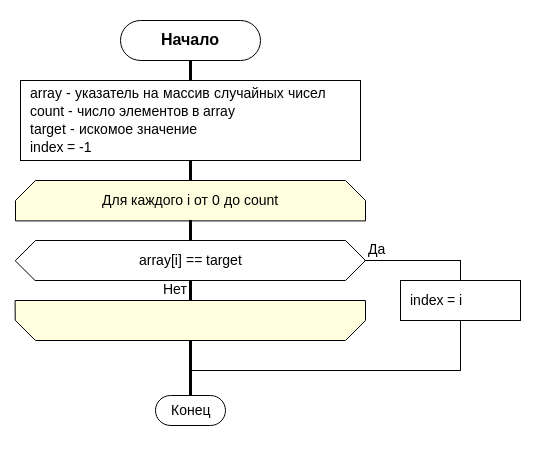
\includegraphics[scale=0.6]{res/flowchart.png}

\subsection{Параллелизация}

Аналогично предыдущей лабораторной работе алгоритм можно параллелизовать, распределив итерации между потоками.
Единственное существенное отличие -- если элемент был встречен, то необходимо в тот же момент выйти из цикла.

Рассмотрим задаваемые опции параллелизации:
\begin{itemize}
    \item \textit{num\_threads} - число используемых потоков;
    \item \textit{shared(array, N, index, target)} - общая для всех потоков память (переменные). Сюда включены массив, его размер, индекс искомого элемента (для сохранения результата) и искомое значение соответсвенно;
    \item \textit{default(none)} - локальность всех переменных, не указанных в \textit{shared}.
\end{itemize}

Для преждевременного прерывания поискового цикла (аналог \textit{break}) будет использоваться \textit{omp cancel for}.
Эта директива прервет все потоки как только искомый элемент будет найден.
Для работы директивы \textit{omp cancel for} может потребоваться установка переменной окружения \textit{OMP\_CANCELLATION=true}.

Также так как используется общая переменная \textit{index}, в операциях с ней следует использовать \textit{omp critical}.
